\documentclass[5p,twocolumn,authoryear]{elsarticle}
\usepackage[T1]{fontenc}
\usepackage{lmodern}
\setlength{\emergencystretch}{1em}
\usepackage{amsmath,amssymb,booktabs,graphicx,array,microtype}
\usepackage{xcolor,hyperref}
\usepackage{dblfloatfix}
\renewcommand{\topfraction}{0.95}
\renewcommand{\dbltopfraction}{0.95}
\renewcommand{\textfraction}{0.05}
\renewcommand{\floatpagefraction}{0.75}
\renewcommand{\dblfloatpagefraction}{0.75}
\setcounter{dbltopnumber}{2}
\usepackage{tikz}
\usetikzlibrary{arrows.meta,positioning,fit,backgrounds}
\hypersetup{colorlinks=true,linkcolor=blue!50!black,citecolor=blue!50!black,urlcolor=blue!50!black}
\newcommand{\todo}[1]{\textcolor{red!70!black}{[TO COMPLETE: #1]}}
\newcommand{\nojepa}{\textsc{NoJEPA}}
\newcommand{\direct}{\textsc{DirectReadout}}
\newcommand{\fullmodel}{\textsc{ForecastAttention}}
\newcommand{\meanmodel}{\textsc{ForecastMean}}
\journal{Medical Image Analysis}
\begin{document}
\begin{frontmatter}
\title{Forecast-aware latent modeling for longitudinal prediction of pathological complete response from breast MRI}
\author{Author information to be completed}
\address{Affiliations and corresponding author to be completed}
\begin{abstract}
Longitudinal breast MRI can reveal treatment response, but endpoint classifiers do not explicitly model the future trajectory implied by an observed history. We investigate forecast-aware latent modeling for pathological complete response (pCR) prediction using three-phase dynamic contrast-enhanced MRI, baseline clinical variables, and assigned-arm scenarios. An autonomous latent predictor estimates future states, and an attention readout combines the predicted terminal state, its change, and direct history features. The cohort comprises 976 patients and 3,641 examinations, with 801 development patients and a fixed internal holdout of 175 patients, including 56 pCR-positive cases. Three matched variants examine direct prediction without future-state supervision, auxiliary-supervised direct prediction, and complete forecast-attention readout. Metrics are averaged over five folds within each training seed and then equally over seeds 21 and 44, yielding one combined estimate. The complete model achieved T0/T1/T2 AUROCs of 0.7323/0.7363/0.7393 and macro AUROC/AP/F1 of 0.7360/0.5969/0.5490, compared with 0.7157/0.5773/0.5333 for the control without future-state supervision. Expanded analysis showed higher sensitivity and NPV but lower specificity and PPV, worse calibration, threshold-dependent net benefit, and heterogeneous subgroup performance. Archived training probes did not indicate uniformly better latent forecasting. Paired patient intervals favored the complete model over the control for macro AUROC, while the incremental forecast-readout interval included zero. These exploratory findings motivate independent validation and a prospectively locked selection policy; the seed pair was selected retrospectively.
\end{abstract}
\begin{keyword}
Breast MRI \sep Pathological complete response \sep Longitudinal imaging \sep Latent dynamics \sep Treatment response prediction
\end{keyword}
\end{frontmatter}
\section{Introduction}
\label{sec:intro}
Neoadjuvant systemic therapy provides an opportunity to monitor breast cancer before surgery and to study how an individual tumor responds over time. Pathological complete response (pCR) is a clinically meaningful endpoint associated with long-term outcomes, although its relationship to prognosis varies across biological subtypes and it should not be equated with a universally valid trial-level surrogate \citep{ctneobc2014}. Predicting pCR from imaging could support response assessment and the design of future adaptive studies. Such a prediction remains a prognostic estimate under an observed treatment context; it does not establish that changing treatment would improve an individual patient's outcome.

Dynamic contrast-enhanced MRI captures three-dimensional anatomy and contrast uptake patterns that evolve during therapy. Prior work in the I-SPY setting has demonstrated associations between MRI-derived tumor measurements and pathological response or subsequent outcomes \citep{hylton2012mri,hylton2016ftv}. Public multicenter imaging resources also make it possible to examine learned representations across repeated visits \citep{tciaispy2_2022,tciaacrin6698_2021}. However, a longitudinal prediction system must operate at the time a decision is considered: a baseline prediction can use baseline information, whereas an interim prediction can use the examination history accumulated by that interim visit. Future scans may inform representation learning on development patients but cannot become inputs to predictions for holdout patients at an earlier landmark.

Most direct classifiers optimize the endpoint of interest from observed images and clinical variables. This is a reasonable objective, but it does not explicitly require the representation to capture how the tumor state may evolve. A different strategy is to predict future imaging information and use the prediction to inform the endpoint readout. Image synthesis provides one route to such a representation, but prediction in a compact latent space can focus the training signal on state evolution without requiring a pixel-space image generator at inference. This distinction is useful for response prediction: the relevant question is whether the learned forecast contributes information to classification, rather than whether a generated image is visually convincing.

Joint-embedding predictive learning offers a general mechanism for predicting target representations computed by a slowly updated encoder \citep{jepa2023}. In a longitudinal medical setting, adapting that principle requires explicit handling of partial histories, missing future observations, treatment context, and the distinction between an auxiliary training target and a classifier input. A model may benefit from a future-state loss while still making a direct prediction from the observed history. Conversely, directly including forecast features in the classifier changes both its information pathway and its parameterization. These effects should be examined through matched controls rather than attributed to a single generic ``world model'' component.

We investigate forecast-aware latent modeling for longitudinal pCR prediction from breast MRI. The model encodes three selected DCE phases at each available visit, fuses observed MRI with baseline clinical information and an assigned treatment-arm scenario, and autonomously rolls the current latent state forward to a terminal stage. A spatial attention mechanism summarizes the predicted terminal state and the predicted change from the current state for pCR classification. We compare the complete model with two direct-readout controls: one without future-state supervision and one with the same auxiliary supervision as the complete model. A supplementary mean-pooling model further examines the attention component.

The study makes three concrete contributions. First, it formulates a common representation and masked future-state objective that can be applied to available T0--T2 histories while using observed later scans only as development-time targets. Second, it provides a staged comparison that distinguishes the effect of auxiliary prediction from the joint effect of forecast readout and attention. Third, it reports landmark-specific discrimination, class-specific errors, calibration, hypothetical decision curves, subgroup heterogeneity, archived forecasting diagnostics, and paired patient-level uncertainty on a fixed internal holdout. The manuscript reports one aggregate obtained by equally averaging seeds 21 and 44 after within-seed fold aggregation. This reporting policy was chosen retrospectively; the analysis remains exploratory, with seed-selection and upstream-independence limits stated explicitly.

\section{Related work}
\label{sec:related}
\paragraph{MRI biomarkers and learned pCR prediction.}
MRI-based response assessment has a substantial clinical and quantitative foundation. Functional tumor volume and related measurements have been studied in longitudinal breast MRI cohorts, including I-SPY \citep{hylton2012mri,hylton2016ftv}. The ACRIN 6698 study additionally examined diffusion-derived measurements in relation to response \citep{ACRIN6698diffusion2018}. These studies motivate imaging-based monitoring but do not establish that a learned model using different inputs or a different evaluation split has equivalent clinical validity. Our experiments use selected DCE phases and baseline clinical variables; diffusion imaging is not an input to the present model.

Learning-based approaches can combine complementary image sequences or repeated examinations. Synthesis-based representation learning has been explored for multi-sequence 3D/4D MRI \citep{han2024synthesis}, and recent studies have examined spatiotemporal or early-treatment information for pCR prediction \citep{tang2025spatiotemporal,du2025early}. Such studies provide relevant methodological context, but differences in patient selection, imaging availability, endpoints, and holdout construction prevent direct numerical comparisons with our results. We therefore do not claim superiority to published systems from cross-paper metric comparisons. Reimplementation of suitable external baselines under the same patient split remains necessary.

\paragraph{Predictive latent representations.}
Predicting a target embedding rather than reconstructing the input image is a central idea in joint-embedding predictive learning \citep{jepa2023}. We use an exponential-moving-average target encoder to define latent states and supervise autonomous future predictions. The present objective is a supervised pCR loss combined with a masked multi-step latent-state loss. It does not activate a separate single-step teacher-forcing JEPA loss, image reconstruction loss, or latent-variance regularizer. This objective-level distinction matters when interpreting the internal experiment name \nojepa{}: that control removes future-state supervision, while retaining the common fusion architecture.

\paragraph{Attention and volumetric image representation.}
Transformer attention provides a flexible way to combine image tokens and contextual information \citep{vaswani2017}. Compact convolutional representations can reduce the cost of processing volumetric MRI, and vector-quantized generative models provide one source of pretrained convolutional encoders \citep{vqgan2021}. Here the pretrained codec contributes a continuous convolutional encoder. The quantizer and image decoder are bypassed, and the main experiments do not synthesize MRI volumes. The final attention weights summarize latent tokens that have already undergone spatial mixing; they are therefore not validated lesion segmentations or anatomical explanations.

\section{Method}
\label{sec:method}
\begin{figure*}[t]
\centering
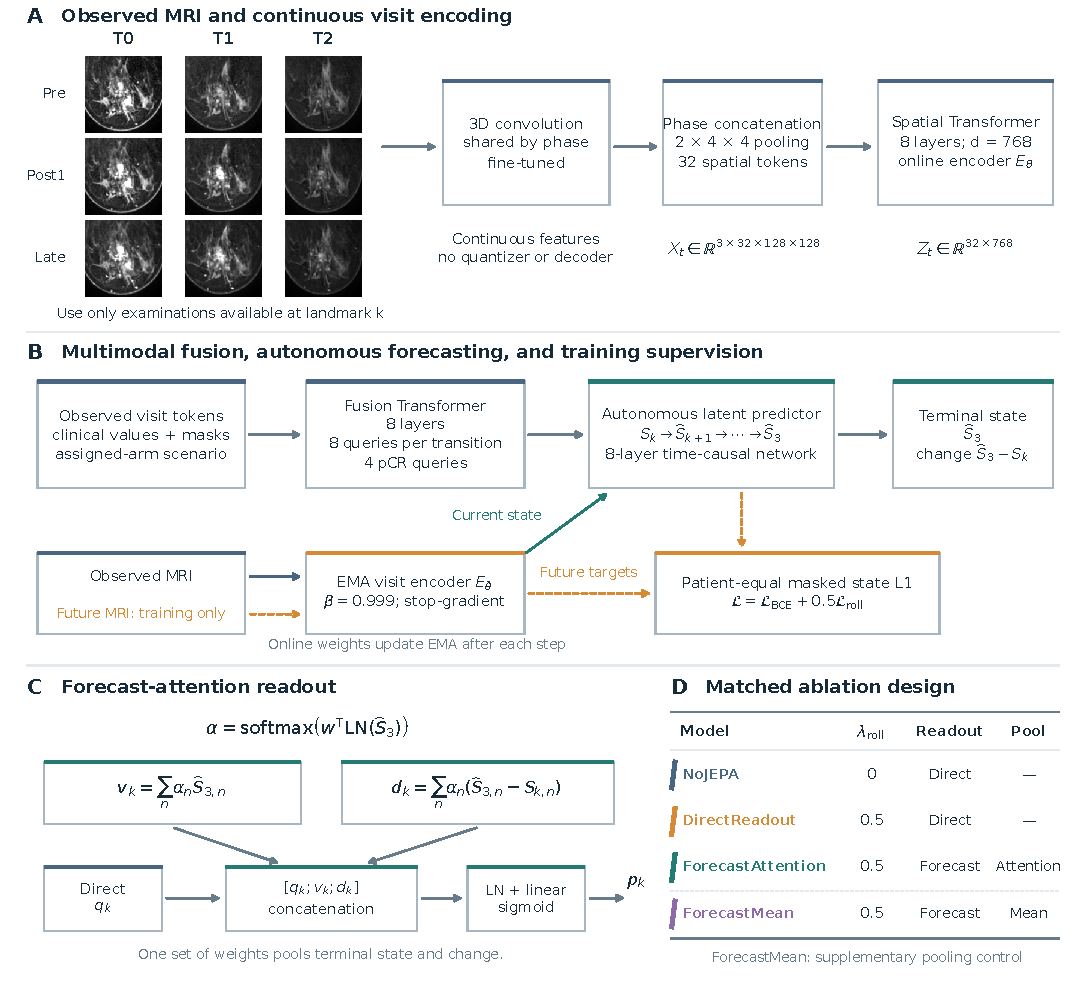
\includegraphics[width=\textwidth]{figures/framework.pdf}
\caption{Forecast-aware latent modeling and matched controls. (A) Real three-phase MRI crops from one development patient illustrate the same baseline-defined plane at T0, T1, and T2; the example and slice were selected without outcomes or model predictions. Only visits available at the prediction landmark are inputs. A shared continuous encoder and spatial Transformer produce visit tokens. (B) Clinical values, availability masks, and an assigned-arm scenario condition fusion and autonomous prediction to T3. The EMA encoder supplies the detached current state; available future MRI supplies training targets only. Dashed orange arrows denote training-target or loss paths. (C) Attention weights pool the predicted terminal state and its change; these features are combined with direct pCR-query features. (D) The primary variants separate removal of future-state supervision from the complete forecast readout. ForecastMean is a supplementary pooling control. MRI tiles are illustrative crops, not generated images, segmentation ground truth, or attention maps.}
\label{fig:framework}
\end{figure*}


\subsection{Longitudinal prediction problem}
\label{sec:problem}
We consider prediction of pathological complete response (pCR) from a patient's available magnetic resonance imaging (MRI) history during neoadjuvant treatment. Canonical examination stages are indexed by $t\in\{0,1,2,3\}$. At a prediction landmark $k\in\{0,1,2\}$, the model receives only examinations acquired and available by that landmark. Let $X_t\in\mathbb{R}^{3\times32\times128\times128}$ denote the processed examination at stage $t$, and let $o_t^{(k)}$ indicate whether this examination is available in the observed prefix. Missing examinations retain their canonical stage rather than shifting later examinations forward. The three channels contain the pre-contrast acquisition, the first post-contrast acquisition, and a metadata-selected late post-contrast acquisition, respectively. The late acquisition is not assumed to have the same acquisition index for all examinations.

The observed information is
\begin{equation}
 \mathcal{H}_k=\bigl\{(X_t,t):o_t^{(k)}=1\bigr\}\cup
 \bigl\{c_k,m_k,a_k,\tau_k\bigr\},
\end{equation}
where $c_k\in\mathbb{R}^{4}$ contains the available clinical variables, $m_k$ their availability indicators, $a_k$ the available assigned treatment-arm category, and $\tau_k$ its declared availability stage. The clinical variables are age at screening, hormone-receptor positivity, HER2 positivity, and a binary MammaPrint variable. Age is standardized using the current training partition; binary variables retain their original coding. Unavailable values are set to zero after standardization and accompanied by an explicit mask. The clinical token embeds the concatenated values and masks. Treatment conditioning uses 13 released arm categories and an additional unknown category. In this retrospective experiment, assigned arm and available baseline clinical variables are assumed to be known at T0. This is an assigned-arm scenario; the categorical input does not specify actual doses, treatment intervals, or treatment changes, and it does not support a causal interpretation.

The output is $p_k=\Pr(y=1\mid\mathcal{H}_k)$, where $y\in\{0,1\}$ is the final pCR label. Future MRI is stored separately as training supervision and is excluded from the prediction input. T3 can provide a future representation target during training, but is never a prediction landmark in the reported T0--T2 protocol.

\subsection{Continuous MRI encoding and multimodal fusion}
\label{sec:encoding}
Each observed examination is encoded independently by an online visit encoder $E_{\theta}$. Its convolutional front end shares the same single-channel weights across the three acquisition phases. Two stride-two three-dimensional convolutional stages, residual blocks, and group normalization produce 64 continuous feature channels per phase at one-quarter input resolution along each spatial axis. The three phase-specific feature maps are concatenated, adaptively averaged to a $2\times4\times4$ grid, and projected to a latent width of $d=768$. This gives $N=32$ spatial tokens per examination. Learned spatial positional embeddings and an eight-layer spatial Transformer then produce the visit representation $Z_t=E_{\theta}(X_t)\in\mathbb{R}^{N\times d}$.

The convolutional front end is initialized from the same pre-existing VQ-GAN-style codec checkpoint for all compared models and is fine-tuned. Here, the model uses continuous features from the codec encoder before its compression projection. It does not use discrete codebook assignments, a quantization objective, a decoder, or adversarial learning during downstream pCR training. \todo{Document the original codec pretraining dataset, patient-level overlap with the present partitions, checkpoint provenance, and applicable redistribution terms.}

Stage embeddings distinguish examination times. Observed image tokens, one clinical token, and one treatment-arm token form the multimodal context. An eight-layer fusion Transformer additionally receives eight learned transition-query tokens for each of the three canonical transitions and four pCR-query tokens. Transition-query slots are retained at every landmark, independently of which future targets happen to be available. Their conditioning is derived entirely from the observed prefix. Context tokens interact bidirectionally; appended transition and pCR queries use a causal attention mask and can attend to the context and preceding query positions. Padding masks remove unobserved image tokens. This produces transition features $A_{j+1}^{(k)}\in\mathbb{R}^{8\times d}$ for transitions $j\rightarrow j+1$, and pCR-query features $Q_k\in\mathbb{R}^{4\times d}$.

All spatial, fusion, and prediction Transformers use pre-normalization blocks, GELU feed-forward layers of width 3072, and dropout 0.3, following the attention-based architecture of \citet{vaswani2017}. Attention has 16 heads with 64 channels per head: its internal width is therefore 1024, followed by projection back to the 768-dimensional residual stream. The clinical and treatment tokens condition forecasting through the shared fusion network rather than through a separately supplied future treatment trajectory.

\subsection{EMA target states and autonomous forecasting}
\label{sec:forecasting}
A target visit encoder $E_{\bar\theta}$ is initialized as a copy of the online encoder and updated after each optimizer step by exponential moving average (EMA):
\begin{equation}
 \bar\theta\leftarrow\beta\bar\theta+(1-\beta)\theta,
 \qquad \beta=0.999.
\end{equation}
The target encoder remains in evaluation mode and receives no gradients. It defines a common representation space for the observed initial state and available future targets,
\begin{equation}
 S_t=\operatorname{stopgrad}\!\left(E_{\bar\theta}(X_t)\right)
 \in\mathbb{R}^{N\times d}.
\end{equation}
Encoding a future target in this branch supplies a loss target only; it does not make that examination available to the forecasting or classification input.

The predictor starts from the latest actually observed state in $\mathcal{H}_k$ and recursively advances to T3. For the reported landmarks, this initial state is $S_k$. At each future transition, it uses the corresponding transition features and its previously generated states. A history input additionally embeds the difference between a source state and its latest available predecessor, with a separate indicator for whether a predecessor exists. Observed history is used where available; after the landmark, the history is extended using model predictions. Thus, a missing future examination removes supervision at that time but does not interrupt the simulated transition sequence.

The prediction network is an eight-layer time-causal Transformer. Each transition block contains its eight transition tokens and 32 spatial source-state tokens, together with learned spatial and temporal embeddings. Tokens can interact within a block; attention between transition blocks is directed from earlier to later blocks. A learned root token remains available when some blocks are masked. The network predicts a residual state increment,
\begin{equation}
 \widehat S_{j+1}=\widetilde S_j+
 G_{\phi,j}\!\left(\widetilde S_{k:j},A_{k+1:j+1}^{(k)},D_{k:j}\right),
 \qquad j=k,\ldots,2,
\end{equation}
where $\widetilde S_k=S_k$, subsequent $\widetilde S_j$ are generated states, and $D_{k:j}$ denotes the available predecessor differences and validity indicators. The residual output projection is initialized to zero, so prediction initially preserves the source state. The transition features summarize the complete legal prefix even when only a subset of previous state differences is available to a particular prediction block.

Forecasts are generated autonomously during training and inference. A true future state never replaces a predicted predecessor. The classifier likewise uses this autonomous trajectory. The configuration includes no teacher-forced next-state loss in these experiments. EMA encoding of real future examinations is used exclusively to evaluate representation error against available targets.

\subsection{Prediction-conditioned pCR readout}
\label{sec:readout}
The full model, \fullmodel{}, combines a direct summary of the observed prefix with summaries of the predicted terminal state and its change from the current state. First, the four pCR-query features are averaged to obtain $q_k=\frac14\sum_{r=1}^{4}Q_{k,r}$. For spatial token $n$, the forecast change is $\Delta S_{k,n}=\widehat S_{3,n}-S_{k,n}$. A learned scalar scorer defines
\begin{equation}
 \alpha_{k,n}=
 \frac{\exp\!\left(w^{\mathsf T}\operatorname{LN}(\widehat S_{3,n})\right)}
 {\sum_{u=1}^{N}\exp\!\left(w^{\mathsf T}\operatorname{LN}(\widehat S_{3,u})\right)}.
\end{equation}
The same weights pool terminal state and change,
\begin{equation}
 v_k=\sum_{n=1}^{N}\alpha_{k,n}\widehat S_{3,n},
 \qquad
 d_k=\sum_{n=1}^{N}\alpha_{k,n}\Delta S_{k,n}.
\end{equation}
The final prediction is
\begin{equation}
 p_k=\sigma\!\left(b+u^{\mathsf T}
 \operatorname{LN}\!\left([q_k;v_k;d_k]\right)\right).
\end{equation}
The scorer is initialized with $w=0$, corresponding to uniform pooling at initialization. Classification gradients propagate through the generated terminal state, predictor, and transition-conditioning pathway. The observed EMA reference state remains detached. The attention weights summarize transformed spatial tokens and should not be interpreted as validated anatomical localization or tumor segmentation.

For \direct{}, pCR is instead predicted directly from $q_k$ using a layer-normalized linear head. Its future-state predictor is trained as an auxiliary task, but generated states are not explicit inputs to the pCR head. The direct head has input width $d$, whereas the full readout has width $3d$. Their comparison therefore evaluates the complete forecast-conditioned readout, including its state and change inputs and classifier width. An additional mean-pooling variant, when reported, retains the forecast-conditioned readout and replaces $\alpha_{k,n}$ by $1/N$.

\subsection{Training objective and matched ablations}
\label{sec:objective}
Let $\mathcal{B}_{y}$ be the labeled patients in a training batch, and let $m_{i,t}^{\mathrm{future}}$ indicate an actually available future target for patient $i$ after its sampled landmark. The pCR objective is unweighted binary cross-entropy,
\begin{equation}
 \mathcal{L}_{\mathrm{pCR}}=
 -\frac{1}{|\mathcal{B}_{y}|}\sum_{i\in\mathcal{B}_{y}}
 \left[y_i\log p_i+(1-y_i)\log(1-p_i)\right].
\end{equation}
Define $M_i=\sum_t m_{i,t}^{\mathrm{future}}$ and $\mathcal{B}_{+}=\{i:M_i>0\}$. Autonomous representation supervision is patient-equal:
\begin{equation}
 \mathcal{L}_{\mathrm{roll}}=
 \frac{1}{|\mathcal{B}_{+}|}\sum_{i\in\mathcal{B}_{+}}
 \frac{1}{M_i}\sum_t m_{i,t}^{\mathrm{future}}
 \frac{\|\widehat S_{i,t}-S_{i,t}\|_1}{Nd}.
\end{equation}
If a batch contains no future targets, this term is zero. Each available future examination has equal weight within a patient; the loss uses no horizon discount, lesion weighting, or fabricated target for a missing visit. Patients without future MRI still contribute pCR supervision.

The full model and \direct{} minimize
\begin{equation}
 \mathcal{L}=\mathcal{L}_{\mathrm{pCR}}+0.5\mathcal{L}_{\mathrm{roll}}.
\end{equation}
\nojepa{} uses the direct pCR head with $\mathcal{L}=\mathcal{L}_{\mathrm{pCR}}$. This historical control name denotes removal of future-state auxiliary supervision, rather than removal of every transition-related module: it retains the shared fusion architecture and transition-query slots. Consequently, \direct{} versus \nojepa{} isolates the added autonomous representation objective under the same direct readout, whereas \fullmodel{} versus \direct{} assesses the added forecast-conditioned classification pathway. The latter comparison cannot isolate spatial attention alone.

All three models omit teacher-forced JEPA, image reconstruction, flow-matching, and variance-regularization losses. In particular, the future objective reported here is autonomous state prediction, despite the JEPA-related implementation lineage. During training, patients are shuffled once per epoch and one actual available T0--T2 landmark is sampled uniformly for each patient. This balances patient contributions without treating a patient with more visits as several independently sampled patients. The same clinical endpoint supervises each sampled prefix; validation assesses all available eligible prefixes using patient-equal weighting.

\section{Dataset and preprocessing}
\label{sec:data}

\subsection{Cohort construction and clinical variables}
We retrospectively analysed longitudinal breast dynamic contrast-enhanced MRI
(DCE-MRI) from the public I-SPY2 and ACRIN-6698 imaging
resources~\cite{tciaispy2_2022,tciaacrin6698_2021}. Source imaging identifiers
were linked to research identifiers using the accompanying official identity
mapping, and outcomes and baseline clinical variables were obtained from the
official I-SPY2 Imaging Cohort~1 clinical spreadsheet. The final cohort
comprised 976 patients with 3,641 usable examinations. Native imaging
identifiers belonged to the ISPY2 and ACRIN-6698 namespaces for 712 and 264
patients, respectively; these identifiers were mapped to the same clinical
release and do not define independent development and external validation
cohorts. The official collection pages identify the source imaging and clinical
release as CC BY 4.0. \todo{Confirm terms for redistributing derived assets and
document the applicable ethics approval or waiver and original consent arrangements.}

Eligibility required an actual baseline examination, an available binary pCR
label, usable baseline registered image assets, and a nonempty baseline
localisation produced by the existing MAMA-MIA segmentation workflow. Of 980
clinically matched source candidates, three lacked a baseline examination and
one had an empty or unavailable predicted baseline localisation. Their
exclusion yielded 976 patients and 3,642 candidate examinations. One
post-treatment examination was subsequently marked unavailable because its
saved within-examination phase transforms displaced the postcontrast images
outside the prescribed baseline crop. The patient's earlier examinations were
retained, leaving 3,641 usable examinations. Missing follow-up examinations did
not cause patient exclusion. No additional admission thresholds based on
normalised cross-correlation, field-of-view ratios, functional tumour volume,
or the availability of an accepted adjacent longitudinal pair were applied.

The endpoint was the released binary pCR field: 313 patients were labelled
positive and 663 negative. \todo{Verify and state the release-specific
pathological definition of pCR, including breast and nodal criteria and the
handling of in-situ disease; do not infer this definition from the binary
column alone.} Baseline covariates were age at screening, hormone-receptor
(HR) status, HER2 status, and the released binary MammaPrint indicator. Age was
available for 973 patients; all three binary covariates were available for the
entire cohort. The official assigned treatment arm, represented by 13
categories, was also supplied to the model. The current experiments use an
\emph{assigned-arm scenario}: the assigned arm and available baseline
covariates are assumed known at baseline. The spreadsheet does not establish
prospective allocation timestamps, doses, cycle-level exposure, or interval
treatment schedules, and the model does not reconstruct these quantities.

\begin{table*}[t]
\centering
\caption{Characteristics of the analysed cohort. Development statistics count
each of the 801 development patients once, rather than pooling overlapping
training folds. Age is reported as mean $\pm$ sample standard deviation among
patients with observed age; other entries are counts.}
\label{tab:cohort}
\small
\begin{tabular}{lrrr}
\toprule
Characteristic & All & Development & Holdout \\
\midrule
Patients & 976 & 801 & 175 \\
pCR positive & 313 & 257 & 56 \\
pCR negative & 663 & 544 & 119 \\
Age (years) & $48.7\pm10.5$ & $48.7\pm10.6$ & $48.9\pm10.2$ \\
Missing age & 3 & 3 & 0 \\
HR positive & 533 & 434 & 99 \\
HER2 positive & 240 & 195 & 45 \\
Available T0 & 976 & 801 & 175 \\
Available T1 & 935 & 760 & 175 \\
Available T2 & 875 & 700 & 175 \\
Available T3 & 855 & 692 & 163 \\
\bottomrule
\end{tabular}
\end{table*}

Examinations were indexed by the canonical study stages T0--T3 rather than
continuous elapsed time. Availability at these stages was 976, 935, 875, and
855 patients, respectively (Table~\ref{tab:cohort}); 803 patients had all four
examinations and 861 had T0--T2. The nominal source protocol acquired T0 before
randomization, T1 after three weeks of the first regimen (paclitaxel with or
without an experimental agent), T2 between paclitaxel and anthracycline
regimens, and T3 after four cycles of anthracycline treatment and before
surgery~\citep{tciaispy2_2022}. Because T0 MRI preceded randomization, supplying
the eventual assigned arm at T0 is a retrospective conditional scenario,
rather than a prospectively available predictor before treatment allocation.
The source protocol used 1.5 or 3.0 Tesla scanners with dedicated breast coils
and required the same scanner configuration within a patient. These are
nominal protocol specifications, not a patient-level audit of timing or
scanner compliance. Twenty-three patients had T0 only and remained
eligible for pCR supervision. Their unavailable future MRI targets were
masked, and no synthetic follow-up images were substituted. Model inputs and
evaluation landmarks were restricted to T0, T1, and T2; a real T3 examination,
when available in the training partition, could provide a future-state target.
\todo{Report the actual examination intervals, acquisition centres, scanner
distribution, and sequence-parameter ranges for the final analysed cohort.}

\subsection{Patient partitioning and evaluation scope}
The cohort was divided into 801 development patients and a fixed internal
holdout of 175 patients, including 56 pCR-positive patients. All holdout
patients had actual T0, T1, and T2 examinations, allowing matched longitudinal
evaluation; 163 also had T3. The holdout retained 139 patients with complete
T0--T2 observations from the historical benchmark and added 36 eligible
patients. Additional patients were selected using outcome quotas and a fixed
baseline-clinical distribution balancing rule with split seed 2026, without
using model predictions or performance. Development folds were stratified by
pCR and examination-availability pattern; rare joint strata were combined
within the same pCR class. Each development patient appeared in validation
exactly once across the five folds. Fold~1 contained 640 training and 161
validation patients; the remaining folds each contained 641 training and 160
validation patients. Training, validation, and holdout identities were
disjoint within each fold, and the same holdout was used for all five trained
models.

This partition is an internal downstream benchmark. In particular, 29 of the
36 added holdout patients had belonged to the development population of an
earlier experiment, so earlier trained models cannot be treated as held out
on the entire new set. The present downstream models were trained using the
new fold definitions. Patient independence of the supplied codec and
segmentation pretraining checkpoints relative to the final holdout has not
yet been established; that provenance must be audited before stronger claims
of end-to-end independence. The complete-examination holdout eligibility also
restricts inference about patients with missing early follow-up examinations.

\subsection{Registration, fixed localisation, and normalisation}
Within each examination, postcontrast phases were registered to the
precontrast reference. Follow-up examinations were aligned to the patient's
T0 reference using the saved longitudinal transforms, retaining a rigid
fallback when the final deformable candidate was not usable. Baseline
localisation used the existing MAMA-MIA nnU-Net prediction on the native
first-postcontrast examination~\cite{mamamia2025}. The centre of the largest
26-connected predicted component defined a fixed baseline crop, which was
reused at every actual follow-up. Follow-up segmentation and follow-up-driven
recentering were not used.

Each examination was represented by three channels: the precontrast phase,
the first postcontrast phase, and the late phase explicitly specified in the
examination metadata. The late channel was not selected by assuming a fixed
phase number or taking the last available phase. Images were resampled to
$32\times128\times128$ voxels with spacing
$2.0\times0.7032\times0.7032\,\mathrm{mm}$ in the slice and two in-plane
dimensions, approximately covering $64\times90\times90\,\mathrm{mm}$.
Linear interpolation was used for MRI intensities and nearest-neighbour
interpolation for masks and acquisition support, with zero padding outside
the acquired field of view. The localisation mask determined the crop; it was
not a contemporaneous ground-truth tumour segmentation or a future
observation supplied to the classifier.

Native metadata, baseline mask headers, registered reference grids, and saved
transforms were maintained as matched versions. Explicit array-index
mappings, rather than placeholder NIfTI affines, defined sampling positions.
The exported arrays were checked for finite values, consistent coordinate
mapping, and numerical agreement after compressed storage and readback.
These checks establish data and geometry consistency but do not establish
anatomical registration or segmentation accuracy. The fixed crop partly
truncated the largest predicted baseline component for 85 patients; these
patients were retained and the limitation was recorded.

Raw cropped intensities were stored once and shared across folds. For each
fold, a single intensity mean and population standard deviation were fitted
to nonzero precontrast foreground voxels from every unique actual examination
of that fold's training patients. The same scalar transform was applied once
to the foreground of all three channels, stages, and partitions; background
and padding remained zero. Validation and holdout images were excluded from
fitting. Age normalisation was likewise fitted to observed training-patient
values; HR, HER2, and MammaPrint retained their official binary coding, with
missingness represented explicitly.

\section{Experimental design}
\label{sec:experiments}
\subsection{Development protocol and landmark evaluation}
The 801 development patients were partitioned into five patient-level folds. Fold 1 used 640 training and 161 validation patients; folds 2--5 each used 641 training and 160 validation patients. The same 175-patient holdout was evaluated by every fold model and every variant. Thus the five test evaluations per variant are repeated evaluations of overlapping trained models on the same patients, rather than five independent test cohorts. Patient identities were disjoint between training, validation, and holdout within the current split.

At each training epoch, a patient contributed one randomly selected available T0, T1, or T2 prefix. Only MRI observations available at or before the selected landmark were classifier inputs. Later observed visits, including T3, could supply latent targets for the auxiliary loss on training patients. Missing targets were masked. The 23 patients with only T0 remained eligible for pCR training but supplied no future-state loss. At evaluation, all three landmarks were evaluated for the 175 holdout patients, each of whom had T0, T1, and T2. T3 was not an evaluation landmark and was not used as observed input for these predictions.

\subsection{Model comparisons}
The principal comparison comprises three variants trained with seeds 21 and 44 and the same five development folds. \nojepa{} uses direct pCR readout and a zero future-state loss weight. \direct{} uses the same direct readout with a future-state loss weight of 0.5. \fullmodel{} retains that auxiliary weight and replaces the direct readout with a concatenation of direct pCR features, attention-pooled predicted terminal state, and attention-pooled predicted change. All variants retain the shared image encoder, clinical inputs, assigned-arm encoding, fusion architecture, and training schedule.

The \direct{}--\nojepa{} contrast most directly tests adding future-state supervision. The \fullmodel{}--\direct{} contrast jointly changes the use of forecast features, spatial pooling, and classifier input width. It cannot isolate attention alone. For that purpose, the supplementary \meanmodel{} comparison uses forecast readout with mean spatial pooling and otherwise matches the forecast-attention configuration. All manuscript-facing results use the same equal aggregation of seeds 21 and 44. No VQ-latent reconstruction-head, change-weighted-loss, or state-conditioned-head variants are included.

\subsection{Implementation and optimization}
The network uses a model width of 768, eight layers in each of the spatial encoder, multimodal fusion module, and predictor, 16 attention heads with 64 dimensions per head, and feed-forward width 3,072. The 1,024-dimensional concatenated attention-head representation is projected back to the 768-dimensional residual stream. The spatial token grid is $2\times4\times4$. The configuration uses eight state queries, four pCR queries, dropout 0.3, and an EMA coefficient of 0.999. The pretrained convolutional encoder is fine-tuned jointly with the remaining network. Its training-patient provenance requires additional documentation, as discussed in Section~\ref{sec:limitations}.

We use AdamW \citep{adamw2019} with an initial base learning rate of $10^{-4}$ for both the encoder and the main network, weight decay 0.05, batch size 16, no gradient accumulation, and gradient-norm clipping at 1.0. Training uses BF16 mixed precision. A ten-epoch warm-up increases the learning rate from $10^{-5}$ to $10^{-4}$, followed by cosine decay to $10^{-6}$ at epoch 100. Training is capped at 200 epochs, with early stopping after 50 epochs without improvement. The best checkpoint is selected independently in each fold using validation patient-equal-prefix F1 at threshold 0.5. This is an F1 selection protocol, even though AUROC is a principal reporting measure. Deterministic execution was not enabled, so a fixed seed does not imply bitwise reproducibility across hardware or software changes.

\subsection{Metrics, aggregation, and patient-level uncertainty}
We report 14 complementary metrics: AUROC, non-interpolated average precision (AP), F1, accuracy, sensitivity, specificity, positive and negative predictive value (PPV/NPV), balanced accuracy, Matthews correlation coefficient (MCC), Youden index, negative log-likelihood (NLL), Brier score, and expected calibration error (ECE) with ten equal-width probability bins. Confusion-matrix counts are additionally retained. Thresholded primary metrics use 0.5. MCC and balanced accuracy help interpret performance under class imbalance~\citep{chicco2020mcc}; positive prevalence is $56/175=0.32$. No holdout threshold optimization or probability recalibration was performed.

Let $M$ denote a metric, $p_{isf\ell}$ the probability for patient $i$, training seed $s$, fold $f$, and landmark $\ell$, and $y_i$ the pCR label. Our single reported landmark summary is
\begin{equation}
\begin{aligned}
 \overline M_{s\ell}&=\frac{1}{5}\sum_{f=1}^{5}M\bigl(\{y_i,p_{isf\ell}\}_{i=1}^{175}\bigr),\\
 \overline M_{\ell}&=\frac{\overline M_{21,\ell}+\overline M_{44,\ell}}{2},\\
 \overline M_{\mathrm{macro}}&=\frac{1}{3}\sum_{\ell=0}^{2}\overline M_{\ell}.
\end{aligned}
\end{equation}
We do not average probabilities across folds or seeds before computing $M$. Each metric is calculated independently in each fitted model; within-seed five-fold means are then equally averaged across seeds. A mean F1 across landmarks is likewise not recomputed after pooling landmark rows. Only the combined two-seed estimate is presented in manuscript figures and tables.

For exploratory uncertainty estimates, we draw 2,000 bootstrap samples of the 175 patients with replacement. Every patient draw is shared across both seeds, all fold models, variants, and landmarks, preserving pairing and repeated observations. Within each resample, metrics are computed separately per fold and then aggregated exactly as above. Percentile 2.5th and 97.5th quantiles form the intervals. They condition on the fitted models and selected analysis; they do not capture retraining, seed-selection, or model-selection uncertainty. Neither ten fitted models nor three repeated landmarks are treated as independent patient samples. We do not make multiplicity-adjusted confirmatory significance claims.

ROC curves are interpolated on a common false-positive-rate grid; PR curves are summarized on a recall grid. Curves and their patient-bootstrap bands follow the same fold-then-seed averaging. Separately calculated mean AUROC/AP values are reported alongside the curves, since interpolation and curve averaging can change the displayed area. Reliability diagrams use five equal-count probability-rank groups within each fitted model, then average corresponding coordinates; these descriptive bins are distinct from the ten fixed bins used for ECE.

\subsection{Operating-point and hypothetical decision analyses}
As a threshold sensitivity analysis, Youden index is maximized on each fold's validation patients separately at T0, T1, and T2. The highest threshold breaks exact ties. That threshold is then fixed for the corresponding holdout evaluation; no holdout prediction chooses it. Bootstrap intervals condition on the fitted threshold rather than refitting it in each resample.

We additionally compute exploratory decision curves~\citep{vickers2006dca}. At risk threshold $q$, the generic positive action is applied when predicted pCR probability is at least $q$. Its mathematical net benefit is
\begin{equation}
 \mathrm{NB}(q)=\frac{\mathrm{TP}(q)}{n}
 -\frac{\mathrm{FP}(q)}{n}\frac{q}{1-q}.
\end{equation}
We calculate this separately for every fitted model over thresholds 0.05--0.80, then apply fold-then-seed aggregation. Treat-all and treat-none are references. The calculation uses uncalibrated probabilities and does not validate a particular escalation, de-escalation, or other management action.

\subsection{Exploratory subgroup and mechanism analyses}
We examine released HR/HER2 combinations, age below or at least 50 years, native source namespace, and saved predicted-component crop coverage. Age 50 is an exploratory reporting cutpoint. Subgroup AUROC/AP are suppressed when fewer than ten patients or fewer than five outcomes in either class are available. Paired within-subgroup patient resampling preserves all seed/fold/landmark pairing; single-class draws are omitted for AUROC intervals and valid-draw counts retained. Intervals are unadjusted, and no subgroup-interaction hypothesis is tested. Source namespaces share the same clinical release and are not independent external cohorts.

Mechanism analysis is restricted to archived fixed-training-probe diagnostics collected every five epochs. These probes sample up to 32 training patients and are not full validation or holdout forecast evaluations. Unlike the missing-target-masked training objective, the archived forecast diagnostic includes only continuous observed visit chains: the real landmark, target, and every intermediate canonical visit must be available. A gap excludes that landmark--target pair, and eligible-patient counts therefore vary by horizon. We report a descriptive common epoch 20 and common-epoch trajectories. Forecast skill is $1-\mathrm{L1}_{\mathrm{forecast}}/\mathrm{L1}_{\mathrm{copy}}$ within the same snapshot's EMA representation; the copy forecast holds the observed landmark state constant. This normalization avoids comparing raw latent errors between separately learned teacher coordinates. Predictor gradient norms from the pCR and weighted rollout objectives are descriptive checks of gradient routing, not independent statistical samples or clinical effects.

\subsection{Scope of the selected-seed-pair analysis}
The choice to average seeds 21 and 44 was made retrospectively after multiple-seed results were available, including holdout results. It was not a prospectively registered seed policy. Using the same pair and weights for every model preserves a matched comparison, but does not remove selection bias or fully characterize training randomness. The analysis is exploratory. A confirmatory study should lock model selection and the seed policy before evaluating independent patients.

\section{Results}
\label{sec:results}
\subsection{Discrimination and the matched model hierarchy}
All 30 principal runs completed training and formal evaluation; the supplementary mean-pooling model contributed ten further completed runs. Forty evaluation receipts and their 120 registered report identities were verified. All holdout evaluations used the same 175 patients and 56 positive labels. Unless stated otherwise, each reported number first averages five fold metrics within a seed, then equally averages seeds 21 and 44. We present one combined estimate per model and landmark.
\begin{table*}[t]
\centering
\small
\caption{Performance on the fixed internal holdout (175 patients, 56 pCR positive). Each value averages five fold metrics within a seed, then equally averages seeds 21 and 44. Macro averages the three landmarks. AP denotes average precision; F1 uses threshold 0.5.}
\label{tab:main}
\begin{tabular}{llrrr}
\toprule
Model & Landmark & AUROC & AP & F1 \\
\midrule
NoJEPA & T0 & 0.7151 & 0.5752 & 0.5334 \\
NoJEPA & T1 & 0.7166 & 0.5815 & 0.5347 \\
NoJEPA & T2 & 0.7154 & 0.5751 & 0.5316 \\
NoJEPA & Macro & 0.7157 & 0.5773 & 0.5333 \\
DirectReadout & T0 & 0.7264 & 0.5863 & 0.5343 \\
DirectReadout & T1 & 0.7285 & 0.5911 & 0.5369 \\
DirectReadout & T2 & 0.7281 & 0.5937 & 0.5562 \\
DirectReadout & Macro & 0.7277 & 0.5904 & 0.5425 \\
ForecastAttention & T0 & 0.7323 & 0.5933 & 0.5391 \\
ForecastAttention & T1 & 0.7363 & 0.5976 & 0.5524 \\
ForecastAttention & T2 & 0.7393 & 0.5998 & 0.5556 \\
ForecastAttention & Macro & 0.7360 & 0.5969 & 0.5490 \\
\bottomrule
\end{tabular}
\end{table*}


\fullmodel{} achieved AUROCs of 0.7323, 0.7363, and 0.7393 at T0, T1, and T2, with AP values of 0.5933, 0.5976, and 0.5998 (Fig.~\ref{fig:discrimination}). Its landmark-macro AUROC/AP/F1 was 0.7360/0.5969/0.5490, compared with 0.7157/0.5773/0.5333 for \nojepa{} and 0.7277/0.5904/0.5425 for \direct{}. The complete model therefore had the highest combined macro values of these three metrics among the principal variants. At T2, however, \direct{} retained a slightly higher F1 (0.5562 versus 0.5556), demonstrating that the ranking is not uniform across metrics and landmarks.

\begin{figure*}[t]
\centering
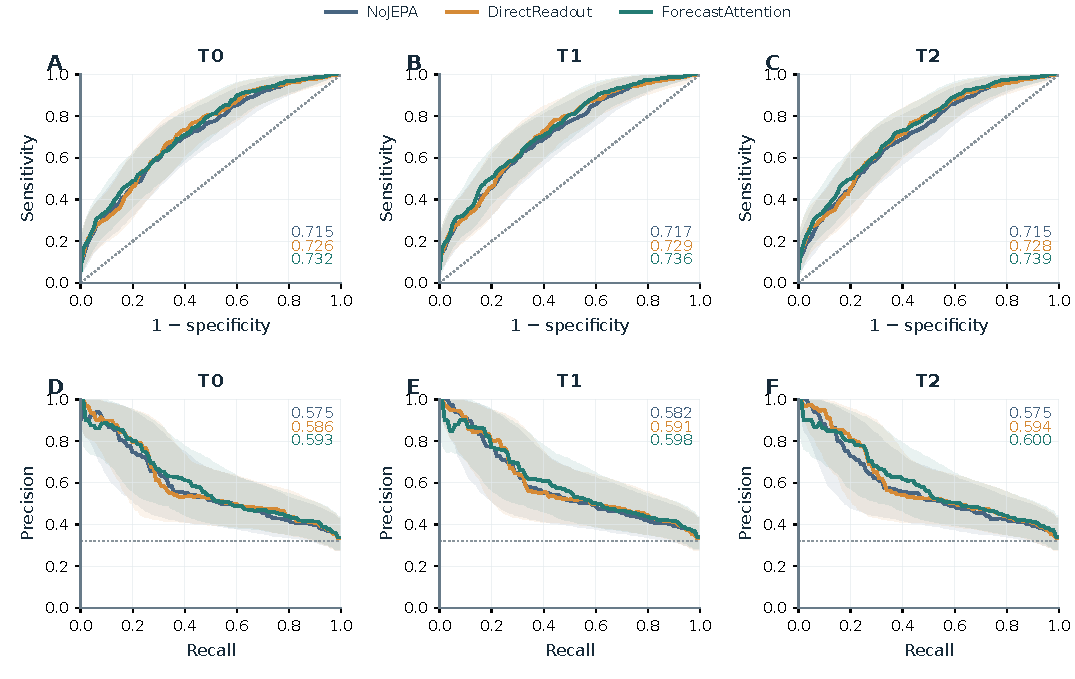
\includegraphics[width=\textwidth]{figures/discrimination.pdf}
\caption{Discrimination across matched landmarks. (A--C) ROC curves; (D--F) precision--recall curves. Curves are calculated separately in each fold model, then averaged within seed and across seeds 21/44. Shading shows pointwise 95\% paired patient-bootstrap intervals conditional on the fitted models. Colored values are the corresponding fold-then-seed mean AUROC or AP; interpolated curve areas need not equal these separately calculated statistics. The dotted PR reference is the 0.32 positive prevalence.}
\label{fig:discrimination}
\end{figure*}

Adding future-state supervision under direct readout increased macro AUROC by 0.0120, AP by 0.0131, and F1 by 0.0092. Adding the complete forecast-attention readout gave a further AUROC increase of 0.0083, AP increase of 0.0065, and F1 increase of 0.0065 relative to \direct{}. The first comparison isolates the auxiliary objective more closely; the second jointly changes the readout information, pooling, and classifier input width. Relative to \meanmodel{}, the full model increased macro AUROC/AP/F1 by 0.0032/0.0092/0.0163 (Table~\ref{tab:pooling}). These descriptive differences do not establish that attention alone causes the complete model's benefit.

Paired patient intervals clarify the strength and limits of these comparisons (Fig.~\ref{fig:paired}). The macro AUROC difference was +0.0203 [0.0042, 0.0381] for \fullmodel{} versus \nojepa{}, and +0.0120 [0.0011, 0.0242] for \direct{} versus \nojepa{}. The additional difference between \fullmodel{} and \direct{} was +0.0083 [$-0.0041$, 0.0215]. AP and F1 differences between the complete model and either direct control had intervals including zero. The intervals condition on retrospectively selected fitted models; exclusion of zero for some AUROC contrasts does not remove selection uncertainty or make this a confirmatory study.

\begin{figure*}[t]
\centering
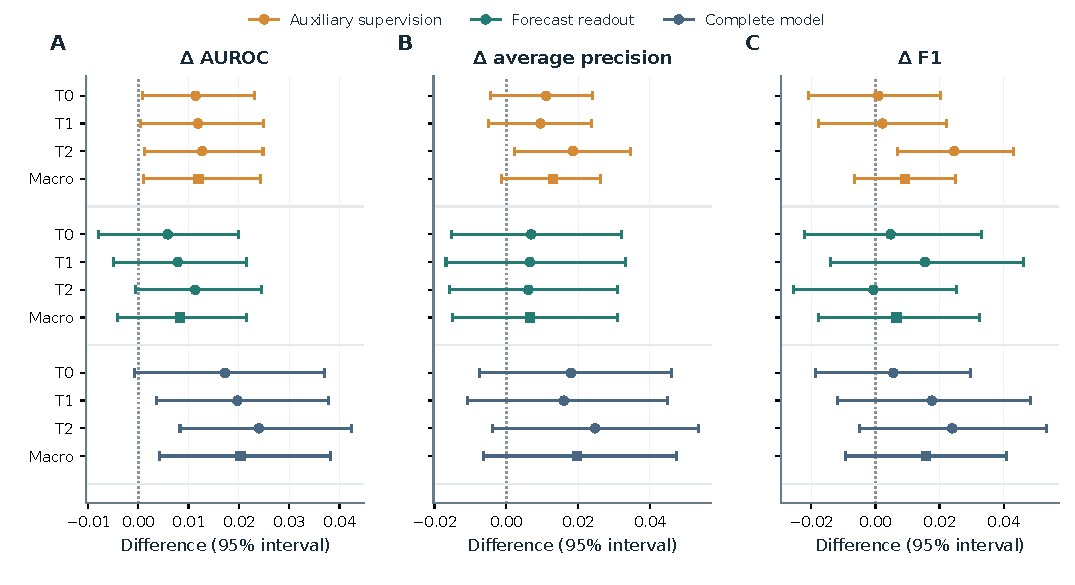
\includegraphics[width=\textwidth]{figures/paired_comparisons.pdf}
\caption{Paired model differences at T0, T1, T2, and the landmark macro. Colors distinguish the auxiliary-supervision contrast, the additional forecast-readout contrast, and the complete-model contrast. Squares denote macro estimates; bars are 95\% patient-bootstrap intervals, with identical patient draws shared across models, folds, seeds, and landmarks. Fold or seed counts are not independent patient sample sizes.}
\label{fig:paired}
\end{figure*}

\subsection{Threshold behavior and class imbalance}
\begin{table*}[t]
\centering
\small
\caption{Extended threshold-dependent metrics at probability threshold 0.5. Values first average five fold metrics within each seed and then equally average seeds 21 and 44 on the same 175 holdout patients; Macro equally averages landmarks. PPV and NPV denote positive and negative predictive value; BA is balanced accuracy.}
\label{tab:extended_operating}
\begin{tabular}{llrrrrrr}
\toprule
Model & Stage & Sens. & Spec. & PPV & NPV & BA & MCC \\
\midrule
NoJEPA & T0 & 0.593 & 0.708 & 0.493 & 0.790 & 0.651 & 0.292 \\
NoJEPA & T1 & 0.580 & 0.727 & 0.501 & 0.788 & 0.654 & 0.298 \\
NoJEPA & T2 & 0.589 & 0.710 & 0.492 & 0.788 & 0.650 & 0.290 \\
NoJEPA & Macro & 0.588 & 0.715 & 0.495 & 0.789 & 0.651 & 0.293 \\
\midrule
DirectReadout & T0 & 0.579 & 0.726 & 0.502 & 0.787 & 0.652 & 0.296 \\
DirectReadout & T1 & 0.589 & 0.716 & 0.497 & 0.788 & 0.653 & 0.295 \\
DirectReadout & T2 & 0.623 & 0.711 & 0.505 & 0.802 & 0.667 & 0.320 \\
DirectReadout & Macro & 0.597 & 0.718 & 0.501 & 0.792 & 0.657 & 0.304 \\
\midrule
ForecastAttention & T0 & 0.629 & 0.674 & 0.485 & 0.803 & 0.651 & 0.295 \\
ForecastAttention & T1 & 0.680 & 0.634 & 0.479 & 0.816 & 0.657 & 0.305 \\
ForecastAttention & T2 & 0.693 & 0.621 & 0.475 & 0.824 & 0.657 & 0.304 \\
ForecastAttention & Macro & 0.667 & 0.643 & 0.480 & 0.814 & 0.655 & 0.301 \\
\bottomrule
\end{tabular}
\end{table*}

Extended metrics reveal a trade-off hidden by AUROC and F1 alone (Table~\ref{tab:extended_operating}). At threshold 0.5, \fullmodel{} had macro sensitivity 0.6673 and NPV 0.8143, compared with 0.5970 and 0.7922 for \direct{}. The increase in sensitivity (+0.0702 [0.0399, 0.1051]) was accompanied by a specificity decrease from 0.7176 to 0.6431 ($-0.0745$ [$-0.0949$, $-0.0554$]) and a PPV decrease from 0.5011 to 0.4796. The full model was therefore more likely to identify pCR-positive patients while also assigning more non-pCR patients a positive prediction.

\direct{} had the highest macro balanced accuracy (0.6573) and MCC (0.3037), compared with 0.6552 and 0.3013 for \fullmodel{} and 0.6513 and 0.2931 for \nojepa{}. Raw macro accuracy was 0.6790, 0.6509, and 0.6743, respectively. Because predicting every patient as non-pCR gives an accuracy of 0.68, accuracy alone does not demonstrate useful discrimination in this imbalanced cohort. Balanced accuracy, class-specific rates, and threshold-free discrimination provide the necessary context.

Validation-selected Youden thresholds did not uniformly improve classification (Table~\ref{tab:extended_threshold}). For \fullmodel{}, sensitivity fell to 0.6405 and specificity increased to 0.6605; macro F1 fell from 0.5490 to 0.5418. The corresponding F1 values changed from 0.5333 to 0.5349 for \nojepa{} and from 0.5425 to 0.5371 for \direct{}. Thus a different validation objective changes the operating point without guaranteeing a higher holdout F1. No holdout labels were used to select these thresholds.

\subsection{Longitudinal information and probability quality}
The same-patient T2--T0 AUROC change was +0.0071 [0.0006, 0.0138] for \fullmodel{}, +0.0003 [$-0.0059$, 0.0067] for \nojepa{}, and +0.0016 [$-0.0038$, 0.0064] for \direct{}. The full model's sensitivity increased from 0.6286 to 0.6929, while specificity decreased from 0.6740 to 0.6210. This illustrates why a positive longitudinal AUROC trend should be considered alongside threshold-dependent errors. Outcome-conditioned score-change distributions are provided in Fig.~\ref{fig:scorechanges}; they average within-model histograms and do not turn the fitted models into a probability ensemble.

\begin{table*}[t]
\centering
\small
\caption{Probability quality averaged across landmarks after fold and seed aggregation. Lower is better. ECE uses ten equal-width bins.}
\label{tab:calibration}
\begin{tabular}{lrrr}
\toprule
Model & NLL & Brier & ECE \\
\midrule
NoJEPA & 0.6018 & 0.2083 & 0.1323 \\
DirectReadout & 0.5959 & 0.2049 & 0.1280 \\
ForecastAttention & 0.6102 & 0.2118 & 0.1544 \\
\bottomrule
\end{tabular}
\end{table*}

The complete model's higher discrimination did not imply better probabilities. Its macro NLL/Brier/ECE was 0.6102/0.2118/0.1544, compared with 0.5959/0.2049/0.1280 for \direct{} and 0.6018/0.2083/0.1323 for \nojepa{}. Reliability curves in Fig.~\ref{fig:calutility} show how observed response frequency relates to predicted probability. The Brier score and ECE of \fullmodel{} worsened toward T2 even as AUROC increased (Fig.~\ref{fig:longitudinal}), reinforcing the distinction between ranking and calibrated probability estimation. Point estimates and conditional patient-bootstrap intervals for all 14 macro metrics are collected in Table~\ref{tab:extended_macro}.

\begin{figure*}[t]
\centering
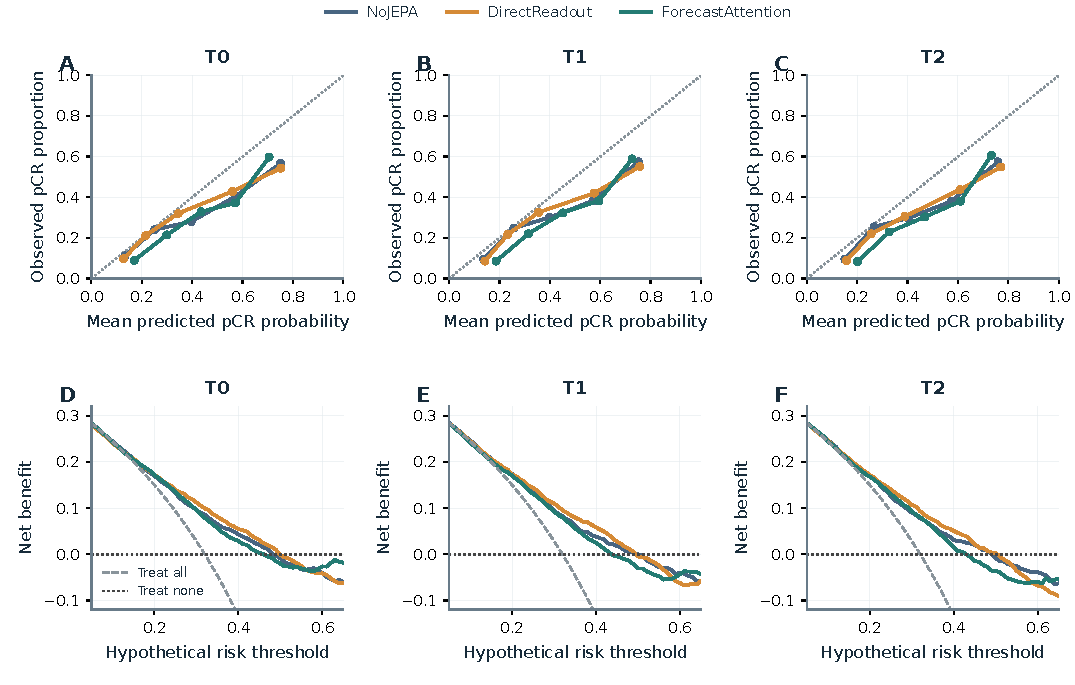
\includegraphics[width=\textwidth]{figures/calibration_utility.pdf}
\caption{Probability quality and hypothetical decision utility. (A--C) Reliability diagrams use five equal-count probability-rank groups within each fitted model (35 patients per group); group coordinates are then averaged over folds and seeds. These groups describe calibration and differ from the ten fixed probability bins used for ECE. (D--F) Net-benefit curves under generic threshold-based positive actions, with treat-all and treat-none references. All curves use the original probabilities, without recalibration. No particular escalation or de-escalation decision is validated by this analysis.}
\label{fig:calutility}
\end{figure*}

\subsection{Hypothetical net benefit}
Decision curves did not preserve the discrimination ranking across thresholds. At a hypothetical risk threshold of 0.30, macro net benefit was 0.1097 for \direct{} and 0.0943 for \fullmodel{}, although the latter had higher AUROC and AP. At threshold 0.50, all three principal models had non-positive macro net benefit relative to the zero reference. These values depend on the mathematical threshold trade-off, pCR prevalence, and the uncalibrated model outputs. They indicate that a ranking advantage alone does not establish a preferable clinical action rule.

\subsection{Exploratory biological and acquisition-related subgroups}
Figure~\ref{fig:subgroups} and Table~\ref{tab:subgroups} show heterogeneity in the combined results. The HR-positive/HER2-negative group contained 68 patients but only 11 pCR-positive cases. Its macro AUROC difference for \fullmodel{} versus \nojepa{} was +0.0522 [0.0095, 0.0995]. In contrast, the HR-positive/HER2-positive group (31 patients, 12 positive) had a difference of $-0.0154$ [$-0.0780$, 0.0473]. The HR-negative/HER2-positive group contained only 14 patients and had a wide interval, while the HR-negative/HER2-negative group had a +0.0219 difference with an interval including zero. These unadjusted subgroup summaries are exploratory, and differences in whether an interval includes zero are not evidence of a subgroup interaction.

The threshold trade-off was also group dependent. In HR-positive/HER2-negative patients, the full model's sensitivity/specificity was 0.2030/0.9170, compared with 0.0970/0.9690 for \nojepa{}. Improved ranking therefore coexisted with low sensitivity at 0.5 in that group. Age-based and source-namespace summaries are descriptive; the two source namespaces belong to the same clinical release and do not form an external validation. Only 11 holdout patients had partial clipping of the largest predicted baseline component, including one positive outcome. AUROC and AP were therefore suppressed for that group under the minimum-outcome rule, rather than interpreting an unstable estimate.

\begin{figure*}[t]
\centering
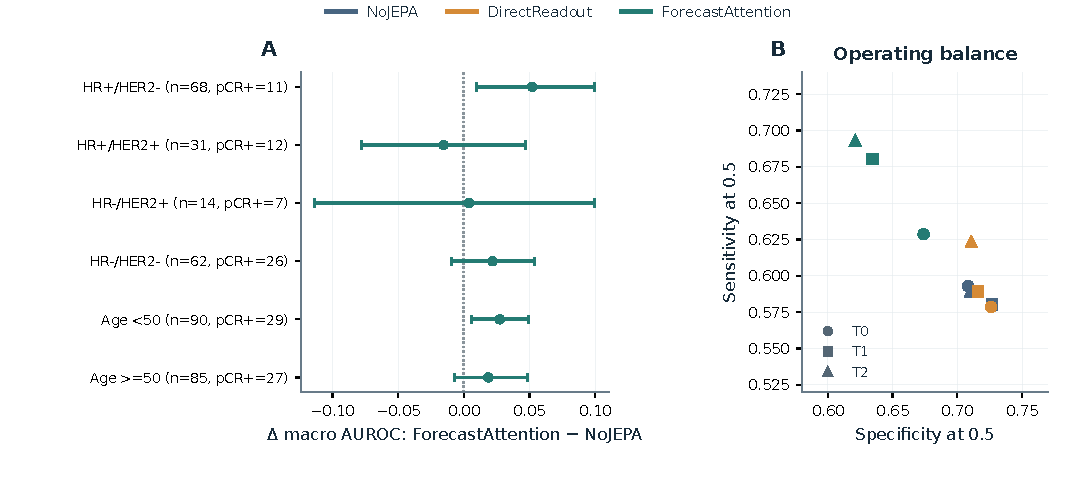
\includegraphics[width=\textwidth]{figures/subgroup_operating.pdf}
\caption{Exploratory heterogeneity and operating-point behavior. (A) Macro AUROC differences between ForecastAttention and NoJEPA within HR/HER2 and age groups, with patient counts, positive-outcome counts, and unadjusted paired intervals. No subgroup-interaction claim is made. (B) Specificity and sensitivity at threshold 0.5, showing the operating-point movement across landmarks. Colors identify models and markers identify landmarks.}
\label{fig:subgroups}
\end{figure*}

\subsection{Archived forecast and gradient diagnostics}
The existing fixed-training-probe archive provides limited mechanistic evidence, distinct from the holdout pCR evaluation (Fig.~\ref{fig:mechanism}). At the illustrative common epoch 20, \direct{} achieved copy-normalized forecast skill of +0.0227, +0.0368, and +0.1584 for one-, two-, and three-step horizons. The corresponding values for \fullmodel{} were $-0.0295$, $-0.0271$, and +0.0174 (Table~\ref{tab:worldprobe}). Consequently, the better pCR ranking of the complete model cannot simply be explained as more accurate latent forecasting under this diagnostic. This diagnostic admits a forecast target only when the landmark, target, and every intervening canonical visit are actually observed; missing intermediate visits exclude that chain. Its eligible population therefore differs by horizon and is narrower than the missing-target-masked training objective. Long-horizon eligibility was only 5--9 patients per training probe, and these measurements are not best-checkpoint holdout forecast accuracy.

The archived task-loss gradient norm in the predictor was zero for \direct{} and averaged 0.8205 for \fullmodel{} at epoch 20; the weighted rollout-gradient norms were 0.1364 and 0.1743, respectively. This supports the expected difference in gradient routing: the full classifier can shape the forecast predictor, while the direct classifier does not read its predicted states. Gradient magnitude itself is not an effect size or evidence that the forecast captures more accurate tumor biology. \nojepa{} has no available world-performance diagnostic and is not assigned an artificial zero error or zero skill.

\begin{figure*}[t]
\centering
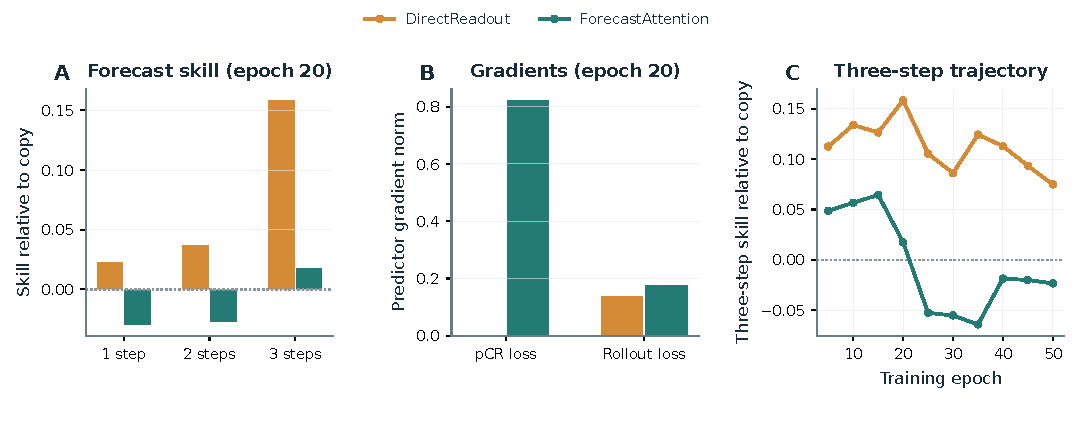
\includegraphics[width=\textwidth]{figures/forecast_mechanism.pdf}
\caption{Archived fixed-training-probe diagnostics. (A) Copy-normalized latent forecast skill at common epoch 20; positive values outperform holding the current state constant in the same snapshot's EMA coordinates. (B) Predictor gradient norms from pCR and weighted rollout losses. (C) Three-step skill over common archived training epochs. Values average folds within seed and then seeds 21/44. Forecast targets require the real landmark, target, and all intermediate visits, so eligibility varies by horizon. These are training diagnostics, not holdout or best-checkpoint mechanism evaluations; three-step eligibility is only 5--9 patients per probe.}
\label{fig:mechanism}
\end{figure*}

\section{Discussion}
\label{sec:discussion}
\subsection{Distinguishing supervision, forecast readout, and forecasting fidelity}
The matched two-seed aggregate supports a descriptive hierarchy in macro discrimination: adding future-state supervision improved direct prediction, and adding the complete forecast-attention readout further improved mean AUROC and AP. Patient-bootstrap intervals for the AUROC contrasts against \nojepa{} excluded zero, while the additional \fullmodel{}--\direct{} interval included zero. The complete-versus-control AUROC gain is larger relative to its conditional uncertainty, whereas the incremental forecast-readout gain remains uncertain. The incremental comparison also changes readout width and pooling, so it does not isolate a single causal mechanism.

The archived forecast probes offer counter-evidence to a simple explanation based on more accurate simulated futures. At common epoch 20, auxiliary-supervised direct prediction had better copy-normalized latent forecast skill than the full classifier, while the full classifier had the better holdout pCR ranking. A predicted representation can therefore be useful to classification without outperforming another model under its own latent reconstruction criterion. One hypothesis is that classification gradients shape the forecast state toward endpoint-relevant directions, at the expense of fidelity to some aspects of the EMA target. The nonzero pCR-to-predictor gradient in the full model is consistent with that information pathway. However, a training probe in a separately learned representation space cannot establish this hypothesis, anatomical forecasting quality, or a causal treatment-response mechanism.

These findings suggest concrete controls for future work: classifier-width-matched direct readout, stopped-gradient forecast features, copy-state readout, and independent holdout forecast evaluation against suitable references. The present main experiments predict embeddings rather than generating MRI for the classifier. The internal control label \nojepa{} also retains the shared fusion architecture and transition queries; it removes the future-state auxiliary objective rather than every world-model-related module. Those distinctions should remain explicit when interpreting the ablation.

\subsection{What additional visits change}
The complete model's AUROC increased across T0--T2 on the same patients, with a paired T2--T0 difference of +0.0071. Its sensitivity increased while specificity decreased. Later histories may help identify patients likely to achieve pCR, but they also move the operating point toward more positive predictions. The outcome-conditioned score histograms describe those score changes; they do not show that every patient's prediction becomes more accurate. Later scans may reveal treatment response, but selection of complete-history patients and the retrospective assigned-arm scenario limit how these patterns can be translated into an earlier decision pathway.

Treatment inputs deserve particular care. T0 imaging preceded randomization in the source protocol, whereas the model is conditioned on the eventual assigned arm. This is a retrospective conditional response estimate, not a deployable prediction before treatment allocation. The encoding does not capture actual delivered dose, cycle timing, dose reductions, adherence, or later changes. Changing the arm token would not identify an individual treatment effect without appropriate causal assumptions and treatment-exposure data.

\subsection{Classification and utility cannot be inferred from AUROC alone}
The expanded metrics show why a higher AUROC does not imply a better decision rule. The full model improved macro sensitivity and NPV but reduced specificity and PPV. Direct readout retained slightly higher balanced accuracy and MCC. At the 0.5 operating point, no principal model exceeded the all-negative reference in macro raw accuracy, although all had balanced accuracy above 0.65 and AUROC above 0.71. Raw accuracy would therefore reward ignoring the positive class in this cohort and should not be the principal assessment criterion.

Validation-selected Youden thresholds altered this trade-off without uniformly increasing holdout F1. Their behavior is consistent with the difference between optimizing balanced class separation and optimizing F1. The full model also had worse NLL, Brier score, and ECE, particularly at later landmarks. Hence its ranking benefit should not be presented as calibrated risk estimation. A clinically motivated endpoint would require calibration fitted without holdout leakage and an operating point justified by the consequences of false-positive and false-negative decisions.

Decision curves reinforce that conclusion: auxiliary-supervised direct readout had greater net benefit than the complete model at some hypothetical thresholds, despite its lower AUROC, and the macro net benefit at 0.5 was non-positive for all principal models. These are mathematical trade-off summaries, not evaluations of a defined clinical intervention. They cannot establish a safe de-escalation strategy or support changing care. External calibration and a prespecified action framework are needed before clinical-utility interpretation.

\subsection{Heterogeneity and the limits of subgroup inference}
Biological subgroup results differed in both ranking and threshold behavior. The HR-positive/HER2-negative group showed a positive macro AUROC difference but still low sensitivity at 0.5. Its low pCR prevalence provides context for predictive values, but does not by itself explain the observed sensitivity. The HR-positive/HER2-positive group had a negative full-versus-control AUROC difference. This negative estimate is relevant evidence against a universal benefit and remains in the report. The small HR-negative/HER2-positive group had too little information for precise conclusions. A subgroup whose interval excludes zero and another whose interval includes zero do not, by themselves, demonstrate a significant interaction.

The source-namespace summaries provide a descriptive acquisition-related check within the same public clinical release; they do not create external validation. Crop sensitivity analysis is similarly limited: only one positive holdout outcome occurred among the 11 patients with partial clipping of the largest predicted baseline component, so a reliable AUROC could not be estimated for that group. The appropriate response is to show the denominator and suppress unstable discrimination rather than report a seemingly precise score.

\subsection{Limitations and a confirmatory study}
\label{sec:limitations}
The seeds 21/44 reporting policy was chosen after results were available. Averaging the same pair across models improves consistency of presentation but does not make selection prospective or exhaust training-randomness uncertainty. Patient intervals condition on the fitted models and, for operating-point analyses, fixed validation-selected thresholds. They do not account for retraining, seed or model selection, threshold-selection uncertainty, or the many exploratory subgroup comparisons. The retrospective two-seed study should therefore be followed by a locked analysis on independent patients.

The holdout is an internal downstream split rather than an independent external institution or prospective cohort. Twenty-nine of its patients had belonged to a development split in an earlier lineage. Current downstream supervised models use the new patient-disjoint folds and are not warm-started from those earlier pCR models, but the pretrained codec and localization model have not yet been fully audited for patient overlap with the current holdout. This prevents a claim that every stage of the pipeline has been evaluated on completely unseen patients.

Fixed T0 localization, registration, and crop coverage are further constraints. Geometry and array checks do not establish anatomical registration accuracy. Some baseline predicted components extend beyond the fixed field of view, and the model may omit multifocal disease or changes outside the crop. Holdout eligibility requires complete T0--T2 imaging, while development retains incomplete histories. Missingness, acquisition variability, and subtype prevalence may therefore affect transportability. The training-probe forecast diagnostics do not replace best-checkpoint holdout mechanism evaluation, and their long-horizon denominators are small.

Finally, the empirical comparison remains an internal architectural ablation rather than a full benchmark against clinical-only, conventional imaging, and independent longitudinal methods. Precise pCR pathology criteria, patient-level scan intervals, ethics determination, and upstream provenance still require final documentation. A stronger study would add matched external baselines, independent validation, a prospectively locked seed policy, anatomical quality review, and externally assessed calibration and clinical operating points.

\section{Conclusion}
We evaluated forecast-aware latent modeling for longitudinal breast-MRI pCR prediction using matched direct and forecast-based controls. Under equal aggregation of seeds 21 and 44 after five-fold metric averaging, the complete model achieved the highest macro AUROC, AP, and F1 among the principal variants. Extended evaluation revealed higher sensitivity and NPV alongside lower specificity and PPV, worse calibration, heterogeneous subgroup behavior, and no uniform net-benefit advantage. Archived training diagnostics did not support explaining the ranking gain simply as more accurate latent forecasting. These exploratory findings motivate independent validation, complete upstream provenance, stronger matched baselines, and prospectively locked model and operating-point selection.

\section*{Data and code availability}
Source imaging collections are available through The Cancer Imaging Archive, subject to their applicable access conditions and licenses. The present derived manifests, processing lineage, and evaluation outputs are retained locally. \todo{Specify the public repository, versioned release, permitted derived-data artifacts, and access mechanism before submission; no public code-release claim is made in this draft.}
\section*{Ethics approval and consent}
\todo{Provide the original studies' ethics and consent statements and the local institutional determination for this secondary analysis, including an approval or exemption identifier where applicable. Public availability alone is not an ethics approval.}
\section*{Funding}
\todo{Provide grant numbers and the funders' roles, or confirm that no specific funding was received.}
\section*{Declaration of competing interest}
\todo{Obtain and insert the actual declarations from every author.}
\section*{CRediT authorship contribution statement}
\todo{Provide author names and agreed contributions; no authorship or contributions have been inferred.}
\section*{Declaration of generative AI and AI-assisted technologies in the manuscript preparation process}
During preparation of this initial draft, OpenAI Codex was used to organize source evidence, generate reproducible aggregate tables and figures, and assist with English drafting. \todo{All authors must review and edit the manuscript, verify every statement and reference, and finalize the disclosure under the journal's current policy before submission.}
\clearpage
\appendix
\section{Supplementary pooling, metrics, and uncertainty}
\label{sec:supplement}
The supplementary \meanmodel{} uses the same training seeds 21/44, folds, observed-history protocol, future-state objective, and forecast classifier feature groups as \fullmodel{}, replacing spatial attention with mean pooling. Only the equal two-seed aggregate is presented, consistent with the main analysis.
\begin{table*}[t]
\centering
\small
\caption{Supplementary pooling comparison using the same two-seed aggregation as the main analysis. ForecastMean and ForecastAttention share forecast readout and future-state supervision, differing in spatial pooling.}
\label{tab:pooling}
\begin{tabular}{llrrr}
\toprule
Model & Landmark & AUROC & AP & F1 \\
\midrule
ForecastMean & T0 & 0.7322 & 0.5863 & 0.5354 \\
ForecastMean & T1 & 0.7339 & 0.5902 & 0.5355 \\
ForecastMean & T2 & 0.7322 & 0.5865 & 0.5273 \\
ForecastMean & Macro & 0.7328 & 0.5877 & 0.5327 \\
ForecastAttention & T0 & 0.7323 & 0.5933 & 0.5391 \\
ForecastAttention & T1 & 0.7363 & 0.5976 & 0.5524 \\
ForecastAttention & T2 & 0.7393 & 0.5998 & 0.5556 \\
ForecastAttention & Macro & 0.7360 & 0.5969 & 0.5490 \\
\bottomrule
\end{tabular}
\end{table*}

\begin{table*}[t]
\centering
\footnotesize
\setlength{\tabcolsep}{5pt}
\caption{All 14 macro metrics for the principal variants: point estimate [95\% patient-bootstrap percentile interval]. Each statistic averages fold metrics within seed, equally averages seeds 21/44, and equally averages T0--T2. Threshold-dependent metrics use 0.5. Identical patient resamples preserve pairing across models, folds, seeds, and landmarks; entries are marginal model intervals, rather than intervals for differences. Intervals condition on the fitted models and exclude retraining and retrospective selection uncertainty. Downward arrows identify metrics for which lower is better.}
\label{tab:extended_macro}
\begin{tabular}{lccc}
\toprule
Metric & NoJEPA & DirectReadout & ForecastAttention \\
\midrule
AUROC & 0.7157 [0.6432, 0.7893] & 0.7277 [0.6560, 0.8007] & 0.7360 [0.6656, 0.8063] \\
AP & 0.5773 [0.4588, 0.6935] & 0.5904 [0.4701, 0.7061] & 0.5969 [0.4841, 0.7136] \\
F1 & 0.5333 [0.4332, 0.6247] & 0.5425 [0.4421, 0.6326] & 0.5490 [0.4598, 0.6319] \\
Accuracy & 0.6743 [0.6168, 0.7307] & 0.6790 [0.6202, 0.7362] & 0.6509 [0.5985, 0.7038] \\
Sensitivity & 0.5875 [0.4780, 0.6994] & 0.5970 [0.4847, 0.7132] & 0.6673 [0.5698, 0.7639] \\
Specificity & 0.7151 [0.6460, 0.7810] & 0.7176 [0.6490, 0.7841] & 0.6431 [0.5770, 0.7076] \\
PPV & 0.4954 [0.3861, 0.6083] & 0.5011 [0.3921, 0.6167] & 0.4796 [0.3817, 0.5831] \\
NPV & 0.7888 [0.7170, 0.8592] & 0.7922 [0.7198, 0.8609] & 0.8143 [0.7456, 0.8797] \\
Balanced accuracy & 0.6513 [0.5860, 0.7171] & 0.6573 [0.5915, 0.7241] & 0.6552 [0.6003, 0.7140] \\
MCC & 0.2931 [0.1656, 0.4208] & 0.3037 [0.1773, 0.4281] & 0.3013 [0.1949, 0.4120] \\
Youden index & 0.3026 [0.1719, 0.4342] & 0.3147 [0.1830, 0.4481] & 0.3104 [0.2005, 0.4279] \\
NLL $\downarrow$ & 0.6018 [0.5403, 0.6624] & 0.5959 [0.5318, 0.6605] & 0.6102 [0.5592, 0.6611] \\
Brier score $\downarrow$ & 0.2083 [0.1825, 0.2347] & 0.2049 [0.1783, 0.2324] & 0.2118 [0.1903, 0.2334] \\
ECE $\downarrow$ & 0.1323 [0.1127, 0.1916] & 0.1280 [0.1101, 0.1868] & 0.1544 [0.1253, 0.2128] \\
\bottomrule
\end{tabular}
\end{table*}

\begin{table*}[t]
\centering
\small
\caption{Exploratory paired patient-bootstrap intervals for three-landmark mean differences (2,000 shared patient draws). Intervals condition on the fitted models and exclude retraining and seed-selection uncertainty.}
\label{tab:bootstrap}
\begin{tabular}{llr}
\toprule
Comparison & Metric & Difference [95\% interval] \\
\midrule
DirectReadout -- NoJEPA & AUROC & +0.0120 [+0.0011, +0.0242] \\
DirectReadout -- NoJEPA & AP & +0.0131 [-0.0013, +0.0261] \\
DirectReadout -- NoJEPA & F1 & +0.0092 [-0.0066, +0.0250] \\
ForecastAttention -- NoJEPA & AUROC & +0.0203 [+0.0042, +0.0381] \\
ForecastAttention -- NoJEPA & AP & +0.0196 [-0.0064, +0.0473] \\
ForecastAttention -- NoJEPA & F1 & +0.0157 [-0.0093, +0.0409] \\
ForecastAttention -- DirectReadout & AUROC & +0.0083 [-0.0041, +0.0215] \\
ForecastAttention -- DirectReadout & AP & +0.0065 [-0.0150, +0.0311] \\
ForecastAttention -- DirectReadout & F1 & +0.0065 [-0.0178, +0.0326] \\
\bottomrule
\end{tabular}
\end{table*}

\begin{table*}[t]
\centering
\small
\caption{Three-landmark mean operating-point sensitivity analysis, equally averaged over seeds 21 and 44 after within-seed five-fold aggregation. The alternative threshold maximizes Youden index separately on each fold and landmark validation set; the highest threshold breaks ties. No holdout predictions select thresholds. Probability-based AUROC and AP are unchanged by this operation.}
\label{tab:extended_threshold}
\begin{tabular}{llrrrr}
\toprule
Model & Policy & F1 & Sens. & Spec. & MCC \\
\midrule
NoJEPA & 0.5 & 0.533 & 0.588 & 0.715 & 0.293 \\
NoJEPA & Validation Youden & 0.535 & 0.614 & 0.684 & 0.285 \\
\midrule
DirectReadout & 0.5 & 0.542 & 0.597 & 0.718 & 0.304 \\
DirectReadout & Validation Youden & 0.537 & 0.601 & 0.706 & 0.298 \\
\midrule
ForecastAttention & 0.5 & 0.549 & 0.667 & 0.643 & 0.301 \\
ForecastAttention & Validation Youden & 0.542 & 0.640 & 0.661 & 0.288 \\
\bottomrule
\end{tabular}
\end{table*}


\begin{figure*}[t]
\centering
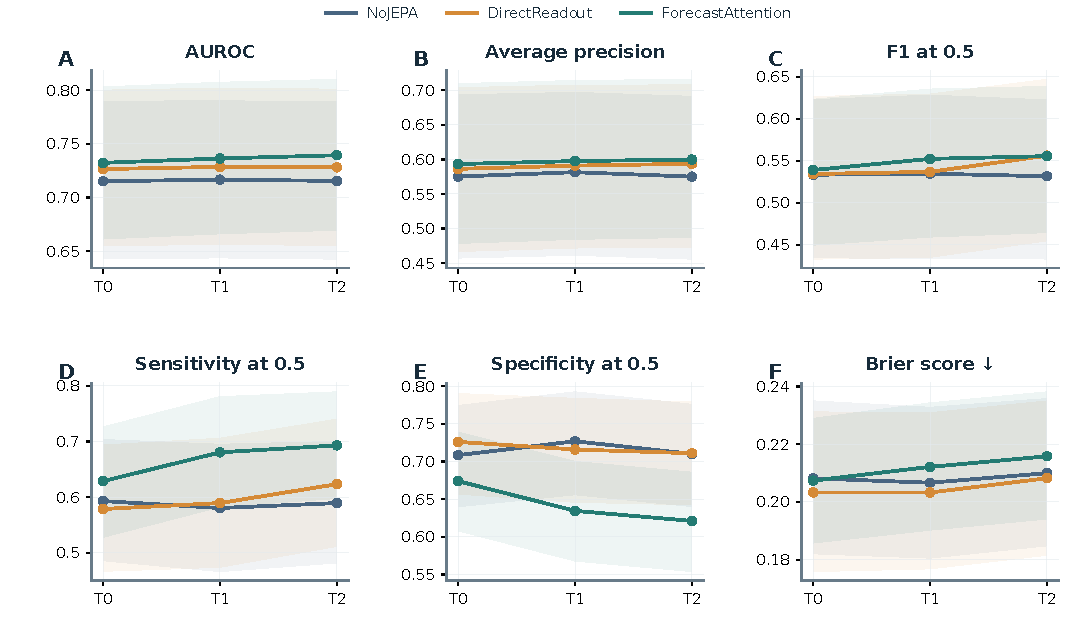
\includegraphics[width=\textwidth]{figures/landmark_performance.pdf}
\caption{Six complementary landmark summaries: AUROC, AP, F1, sensitivity, specificity, and Brier score. All points use fold-then-seed aggregation; shading is the conditional 95\% patient-bootstrap interval. The same 175 patients appear at every landmark. A trend in ranking can coexist with a different trend in calibration or error types.}
\label{fig:longitudinal}
\end{figure*}

\begin{figure*}[t]
\centering
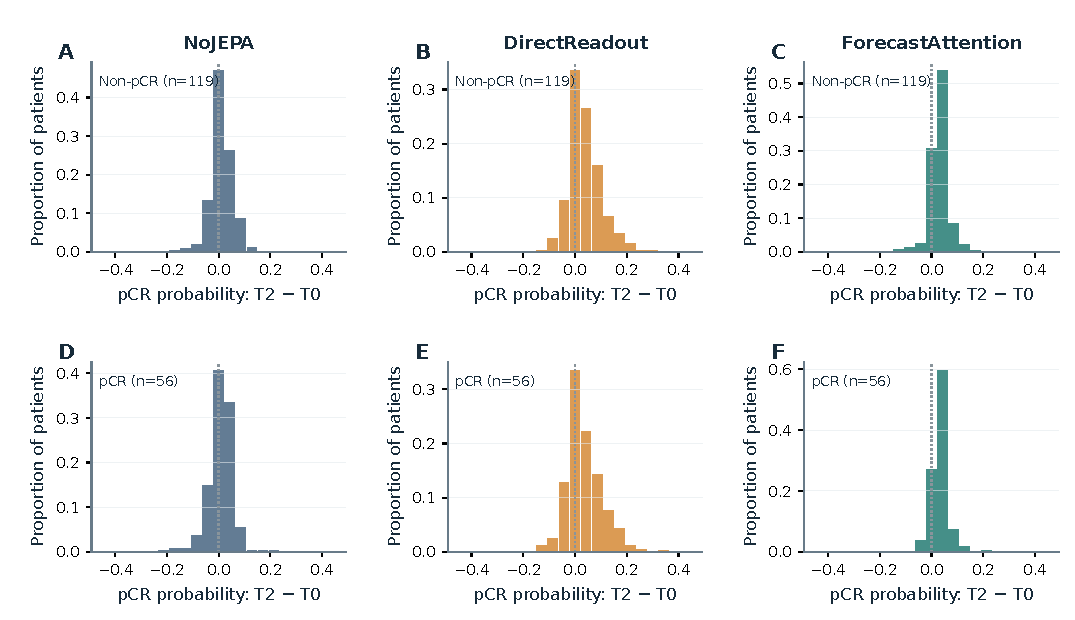
\includegraphics[width=\textwidth]{figures/outcome_score_changes.pdf}
\caption{Outcome-conditioned changes in predicted pCR probability from T0 to T2. Panels separate models and outcome classes. Histograms are computed within each fitted model and then averaged over folds and seeds; they are not histograms of probability-ensemble predictions. Changes describe model scores and do not establish an individual treatment effect.}
\label{fig:scorechanges}
\end{figure*}

\section{Supplementary subgroup and training-probe summaries}
\begin{table*}[t]
\centering
\small
\caption{Exploratory subgroup discrimination for the equal-weight seeds 21/44 mean. AUROC is averaged over five folds within each seed, then seeds 21/44 equally, and T0--T2; intervals are paired patient-bootstrap intervals for ForecastAttention minus NoJEPA, conditional on the fixed models. Age 50 is an exploratory reporting cutpoint. Namespace groups are parts of one clinical release, not external cohorts.}
\label{tab:subgroups}
\begin{tabular}{lrrr}
\toprule
Subgroup ($n$/pCR+) & NoJEPA & Full & $\Delta$ AUROC [95\% interval] \\
\midrule
HR+/HER2- (68/11) & 0.659 & 0.711 & +0.052 [+0.009, +0.099] \\
HR+/HER2+ (31/12) & 0.636 & 0.621 & -0.015 [-0.078, +0.047] \\
HR-/HER2+ (14/7) & 0.812 & 0.816 & +0.004 [-0.113, +0.099] \\
HR-/HER2- (62/26) & 0.632 & 0.654 & +0.022 [-0.009, +0.054] \\
Age $<$50 (90/29) & 0.658 & 0.685 & +0.027 [+0.006, +0.049] \\
Age $\geq$50 (85/27) & 0.774 & 0.793 & +0.019 [-0.007, +0.049] \\
ISPY2 namespace (125/39) & 0.674 & 0.692 & +0.018 [-0.003, +0.042] \\
ACRIN-6698 namespace (50/17) & 0.826 & 0.851 & +0.025 [-0.001, +0.057] \\
\bottomrule
\end{tabular}
\end{table*}

\begin{table*}[t]
\centering
\small
\caption{Archived epoch 20 fixed-training-probe diagnostics, averaged within each seed over five folds and then equally over seeds 21/44. Skill is $1-\mathrm{L1}_{forecast}/\mathrm{L1}_{copy}$ within the corresponding EMA coordinates; positive is better than holding the landmark state constant. These are training-probe summaries, not best-checkpoint holdout forecast evaluations. NoJEPA has no trained-world diagnostic.}
\label{tab:worldprobe}
\begin{tabular}{lrrr}
\toprule
Model & Horizon 1 skill & Horizon 2 skill & Horizon 3 skill \\
\midrule
NoJEPA & -- & -- & -- \\
DirectReadout & +0.023 & +0.037 & +0.158 \\
ForecastAttention & -0.029 & -0.027 & +0.017 \\
\bottomrule
\end{tabular}
\end{table*}


\section{Reproducibility and reporting items to complete}
The source package includes aggregate CSV files, source-report hashes, reproducible metric and figure scripts, the bootstrap procedure, and the official article class. It contains no patient identifiers, patient-level prediction rows, original MRI volumes, or model checkpoints. The method figure includes only rendered, anonymous development-image slices. Training seeds 21 and 44 are averaged equally after within-seed fold aggregation. Seed-specific aggregates are retained for numerical audit but are not separate manuscript results.

\todo{Before submission, complete author and ethics statements; verify the precise pCR pathology definition; document codec and segmentation patient-level pretraining provenance; add matched external baselines and a prospectively locked seed-selection policy; audit external-cohort independence; and confirm the journal's current submission and anonymization requirements.}

\clearpage
\bibliographystyle{elsarticle-harv}
\bibliography{references}
\end{document}
